%プログラミング応用/ソフトウェア工学 要求仕様書 要求仕様書
\documentclass[11ptm]{jsarticle}

\usepackage{etoolbox}

\usepackage{array}

\usepackage{enumitem}

\usepackage{amsmath, newtxmath}

\usepackage[dvipdfmx]{graphicx}
%\usepackage[draft, dvipdfmx]{graphicx}

\usepackage[hang, small, bf]{caption}
\usepackage[subrefformat=parens]{subcaption}
\captionsetup{compatibility=false}

\usepackage{listings, jlisting}

\lstset{
  basicstyle={\ttfamily\small},
  frame=tbrl,
  breaklines=true,
%  language=C,
  lineskip=-0.5ex,
  tabsize=2
}


\usepackage{tabularx}

\usepackage{multirow}

%\usepackage[subrefformat=parens]{subcaption}


\makeatletter
\AtBeginDocument{
\let\c@figure\c@lstlisting
\let\thefigure\thelstlisting
\let\ftype@lstlisting\ftype@figure
}
\makeatother

\title{{\Huge 要求仕様書}\\第6版}
\author{24 高橋祥吾\\26 田桑大輔\\29 田中稀尋\\30 谷川僚}
\date{}

%%%%%%%%%%%%%%%%%%%
%%%%%%%%%%%%%%%%%%%
\begin{document}

\setcounter{page}{0}

\maketitle
\thispagestyle{empty}

\clearpage

\setcounter{page}{0}
\thispagestyle{empty}

\tableofcontents
\clearpage


%%%%%%%%%%%%
%\clearpgae
\section{ソフトウェアの概要}
\label{sec:ソフトウェアの概要}
本節では, POaM資産管理システム(仮称)の概要を述べる.

%%%%%%
%\clearpage
\subsection{はじめに}
\label{subsec:はじめに}
本ソフトウェアはサレジオ高専で備品を扱う際に使用するソフトウェアである. \par
サレジオ高専での備品の管理は10,000円以上のものを対象に行われており, 対象の備品にID, 種類, 名前, 管理者が書かれたシールを貼り管理している. 現状では備品を管理する際にリストへの追加や削除が簡単に行えないのに加え, 備品が移動した際に再度の登録を行っていないため, 備品の紛失などが起こってしまっている.\par
これを防ぐために, PCやスマートフォンなどの各種端末から容易にアクセス可能で, 備品の情報を簡単に閲覧・更新できるようなソフトウェアを作成する.

%%%%%%
%\clearpage
\subsection{作成するソフトウェアの全体像}
\label{subsec:作成するソフトウェアの全体像}
\ref{subsec:はじめに}節で挙げた問題点を技術的に解決できるようなソフトウェアを作成するために, 以下に表されるような項目の実装が必要だと考えている.
\begin{itemize}
  \item 備品データを視覚的に管理・検索・追加・削除・変更を行えるようなプラットフォーム
  \item 備品データを効率的に管理するデータベース
  \item 簡潔明瞭なインターフェース
  \item ユーザ機能(管理者ユーザ, 一般ユーザ)
  \item QRコードなどを活用した, カメラ付き端末からのアクセス
\end{itemize}


%%%%%%%%%%
\clearpage
\section{開発及び動作プラットフォーム}
\label{sec:開発及び動作プラットフォーム}
本ソフトウェアの開発及び動作をするプラットフォームを以下に示す.

%%%%%
%\clearpgae
\subsection{ソフトウェアの開発環境}
\label{subsec:ソフトウェアの開発環境}
\begin{description}[labelwidth=9em]
  \item[使用言語] HTML, CSS, JavaScript, PHP, MySQL
  \item[使用フレームワーク] XAMPP
  \item[使用ミドルウェア] Git
  \item[使用開発環境] Visual Studio Code, Xcode
\end{description}

\subsection{ソフトウェアの動作プラットフォーム}
\label{subsec:ソフトウェアの動作プラットフォーム}
本ソフトウェアは, インターネットに接続可能で, ブラウザがインストールされている各種端末上で動作する. \par
スタンドアロン(オフライン)でも動作するようにするか, オンライン上での動作に限定するかは未定である.
%\begin{itemize}
%\item ブラウザがインストールされている各種端末
%\end{itemize}


%%%%%%%%%%
\clearpage
\section{ソフトウェア全体の構成}
\label{sec:ソフトウェア全体の構成}
本ソフトウェアは, サーバ・クライアント方式のWebアプリケーションでの実装を想定している. そのため, ユーザが操作するWebページとサーバ上のデータベースが存在し, 互いに連携する. \par
\ref{subsec:ソフトウェアの開発環境}節より, それぞれのサイドでは次の言語および開発環境を使用する予定である.
\begin{description}[labelwidth=15em]
  \item[クライアントサイド(Webページ)] HTML, CSS, JavaScript
  \item[サーバサイド] PHP, MySQL
\end{description}
また本ソフトウェアは, \ref{subsec:作成するソフトウェアの全体像}節で挙げた項目において対応する機能およびシステムによって構成される. 対応表を以下に示す.
\begin{table}[h]
  \caption{必要項目に対応する機能}
  \label{tb:必要項目に対応する機能}
  \centering
  \begin{tabularx}{\linewidth}{l|l}
    備品データを視覚的に管理・検索・追加・削除・変更を   & \multirow{2}{*}{登録機能, 削除機能, 変更機能, 検索機能} \\
    行えるようなプラットフォーム                         &                                                         \\
    \hline
    備品データを効率的に管理するデータベース             & サーバによるデータベース                                \\
    \hline
    簡潔明瞭なインターフェース                           & Webページ                                               \\
    \hline
    ユーザ機能(管理者ユーザ, 一般ユーザ)                 & ユーザ登録・ログイン機能                                \\
    \hline
    QRコードなどを活用した, カメラ付き端末からのアクセス & 未定                                                    \\
  \end{tabularx}
\end{table}


%%%%%%%%%%
\clearpage
\section{各機能・システムの詳細}
\label{sec:各機能の詳細・システムの詳細}
各機能および各システムについての詳細を以下にまとめる.

%%%%%
%\clearpage
\subsection{データの形式}
\label{subsec:データの形式}
本ソフトウェアは資産情報をデジタルデータで扱っていく. この際に必要になる情報の保存形式を次の表\ref{tb:データの形式}に示す.
\begin{table}[h]
  \caption{データの形式}
  \label{tb:データの形式}
  \centering
  \begin{tabular}{@{}l|l|l|l|l@{}}
    項目     & 概要                               & 要求する入力形式     & 登録の可不可 & 変更の可不可 \\
    \hline\hline
    資産番号 & 資産ごとの固有のID                 & システムで生成       & admin        & admin        \\
    \hline
    資産名   & 登録する際の名称. 型番など.        & 文字列               & possible     & admin        \\
    \hline
    形式     & 資産の分類. PCやプリンターなど     & 選択形式または文字列 & possible     & admin        \\
    \hline
    所属     & 資産が利用, 所在する所属. 学科など & 選択形式             & possible     & admin        \\
    \hline
    場所     & 資産の所在. 部屋番号を想定         & 選択形式             & possible     & possible     \\
    \hline
    担当     & 資産の所有者および使用者           & 文字列               & possible     & possible     \\
    \hline
    管理者   & 資産の管理者または責任者           & 選択形式または文字列 & possible     & admin        \\
    \hline
    個数     & 資産の個数                         & 整数値               & possible     & possible     \\
    \hline
    画像     & 資産の写真またはイメージ図         & 画像のアップロード   & possible     & admin        \\
    \hline\hline
    取得日時 & 資産情報を登録した日時             & システムで生成       & impossible   & impossible   \\
    \hline
    編集日時 & 資産情報に変更を加えた最新の日時   & システムで生成       & impossible   & impossible
  \end{tabular}
\end{table}\par
変更の可不可について, 変更可能性は低いが修正する可能性があるものを, 管理者ユーザによってのみ変更可能であるとして, adminと表記した.\par
個数については, 変更時に任意の量だけ場所の変更などが可能で, 場所が異なる資産については別のデータとして管理されるようになる.

%%%%%
%\clearpage
\subsection{一般ユーザと管理者ユーザについて}
\label{sec:一般ユーザと管理者ユーザについて}
一般ユーザと管理者ユーザの概要や相違点などについて記述する. \par
一般ユーザはデータの登録(資産番号を除く), 資産の場所・担当・個数の変更が可能である. 管理者ユーザの管理下にあり, 管理者ユーザ以外が一般ユーザを新規登録することはできない.

%%%%%
\clearpage
\clearpage
\subsection{状態遷移図}
\label{sec:状態遷移図}
本ソフトウェアを実行した際の状態遷移図を次に示す. 図\ref{fig:一般ユーザの状態遷移図}を一般ユーザの状態遷移図, 図\ref{fig:管理者ユーザの状態遷移図}を管理者ユーザの状態遷移図とする.
\begin{figure}[h]
  \centering
  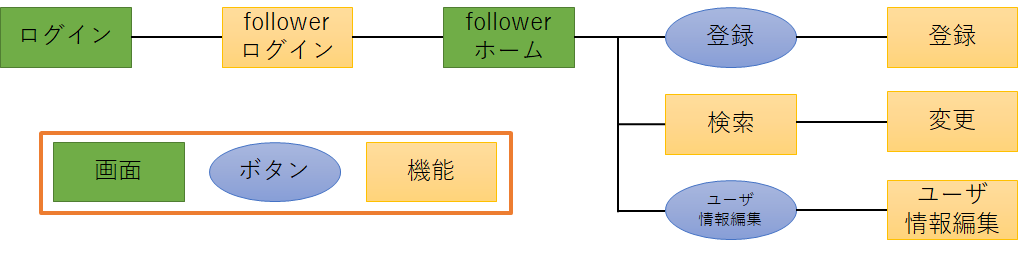
\includegraphics[keepaspectratio, width=0.68\linewidth]{source/follower_transition_diagram.png}
  \caption{\label{fig:一般ユーザの状態遷移図}一般ユーザの状態遷移図}
\end{figure}
\begin{figure}[h]
  \centering
  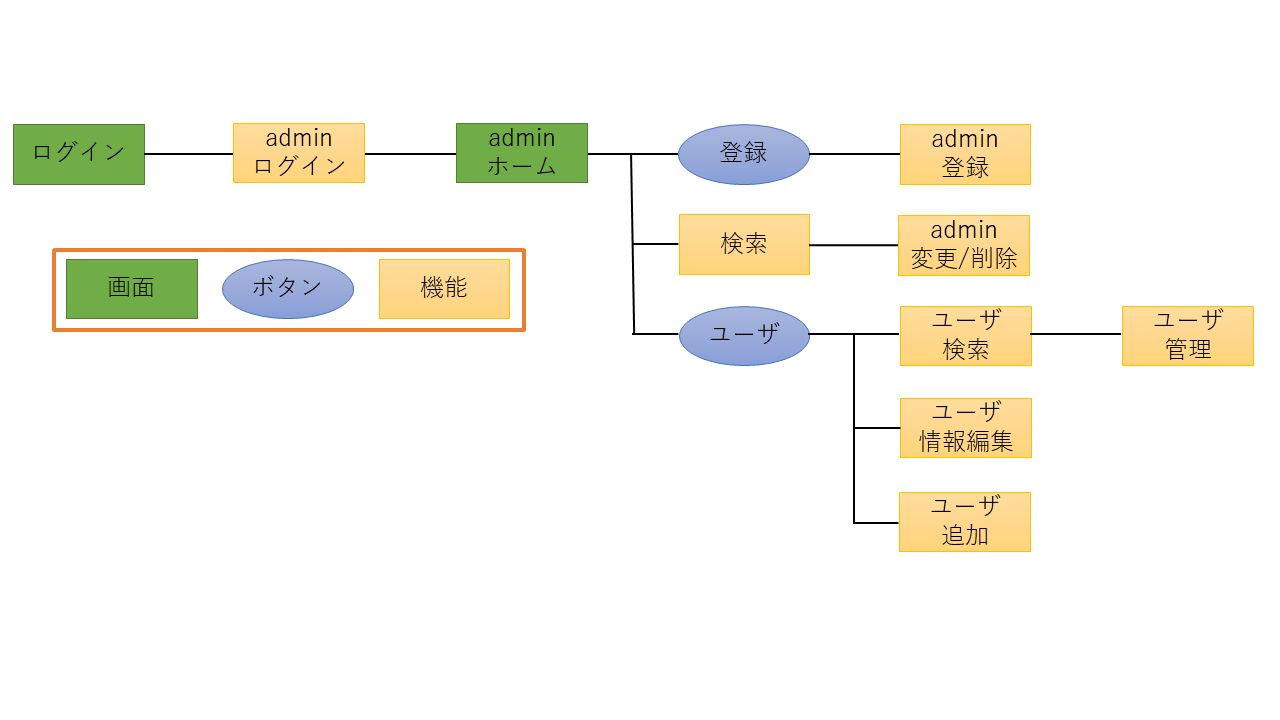
\includegraphics[keepaspectratio, width=0.8\linewidth]{source/admin_transition_diagram.png}
  \caption{\label{fig:管理者ユーザの状態遷移図}管理者ユーザの状態遷移図}
\end{figure}
各画面および機能の参照先を次に示す.
\begin{table}[h]
  \caption*{参照先}
  %\label{tb:}
  \centering
  \begin{tabular}{c|c}
    ログイン                   & \ref{sec:ログイン画面}節 図\ref{fig:ログイン画面のイメージ図}                                                                                                             \\
    \hline
    ホーム                     & \ref{sec:ホーム画面}節 図\ref{fig:ホーム画面(一般ユーザ)のイメージ図}, \ref{fig:ホーム画面(管理者ユーザ)のイメージ図}                                                     \\
    \hline
    登録                       & \ref{sec:新規登録画面}節 図\ref{fig:新規登録画面(一般ユーザ)のイメージ図}, \ref{fig:新規登録画面(管理者ユーザ)のイメージ図}                                               \\
    \hline
    検索                       & \ref{sec:ホーム画面}節 図\ref{fig:ホーム画面(一般ユーザ)のイメージ図}, \ref{fig:ホーム画面(管理者ユーザ)のイメージ図}                                                     \\
    \hline
    変更                       & \ref{sec:情報変更画面}節 図\ref{fig:情報変更画面(一般ユーザ)のイメージ図}, \ref{fig:情報変更画面(管理者ユーザ)のイメージ図}                                               \\
    \hline
    ユーザ情報編集             & \ref{sec:ユーザ情報編集画面・ユーザ管理画面}節 図\ref{fig:ユーザ情報編集画面のイメージ図}                                                                                 \\
    \hline
    ユーザ検索・管理・新規作成 & \ref{sec:ユーザ情報編集画面・ユーザ管理画面}節 図\ref{fig:ユーザ管理画面のイメージ図}, \ref{fig:個別ユーザ管理画面のイメージ図}, \ref{fig:ユーザ新規作成画面のイメージ図}
  \end{tabular}
\end{table}



%%%%%
\clearpage
\subsection{イメージ図}
\label{sec:イメージ図}
状態遷移図(図\ref{fig:一般ユーザの状態遷移図}, \ref{fig:管理者ユーザの状態遷移図})内にある各画面の完成イメージを以下に示していく.

%%%%%
%\clearpage
\subsubsection{ログイン画面}
\label{sec:ログイン画面}
メールアドレス(サレジオドメイン)に基づく{\bf ID}と任意に設定する{\bf パスワード}を入力し, ログインする. \par
ログインすることによって誰がどのように資産データに変更を加えたかのログを残すことができるため, ユーザおよびログインのシステムを導入した.
\begin{figure}[h]
  \centering
  \fbox{
    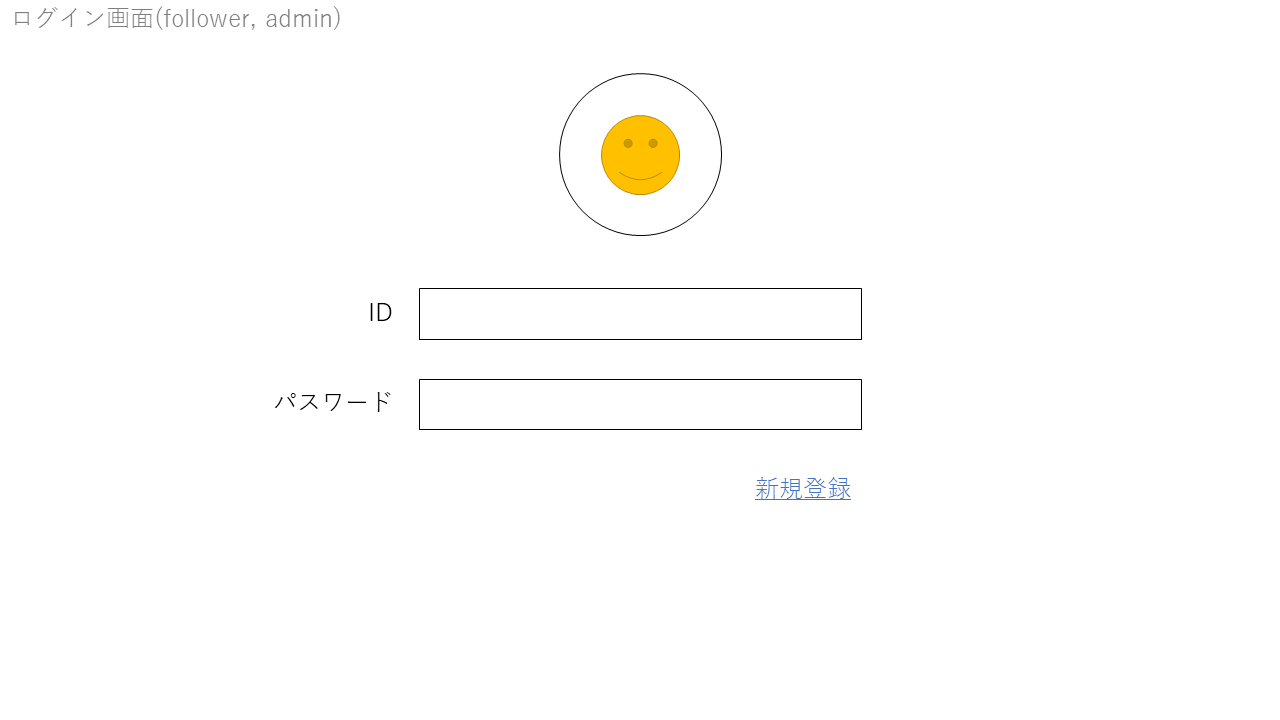
\includegraphics[keepaspectratio, width=0.8\linewidth]{source/login.PNG}
  }
  \caption{\label{fig:ログイン画面のイメージ図}ログイン画面のイメージ図}
\end{figure}

%%%%%
\clearpage
\subsubsection{ホーム画面}
\label{sec:ホーム画面}
図\ref{fig:ホーム画面(一般ユーザ)のイメージ図}が一般ユーザ, 図\ref{fig:ホーム画面(管理者ユーザ)のイメージ図}が管理者ユーザに表示されるホーム画面のイメージ図である. \par
システムロゴ, 資産登録機能へジャンプするボタン, ユーザ情報編集機能(一般ユーザ)またはユーザ管理機能(管理者ユーザ)へジャンプするボタン, 資産検索機能を備えている. 検索機能では, 特定のデータ項目における絞り込みでの検索が可能で, 項目を選択することで動的に資産を見つけることができる. \par
UIの違いはないが, ログインしたあとすぐに表示される画面であることから, どちらの権限を持つアカウントでログインしたかを分かりやすくするために異なる配色を用いた.
\begin{figure}[h]
  \centering
  \fbox{
    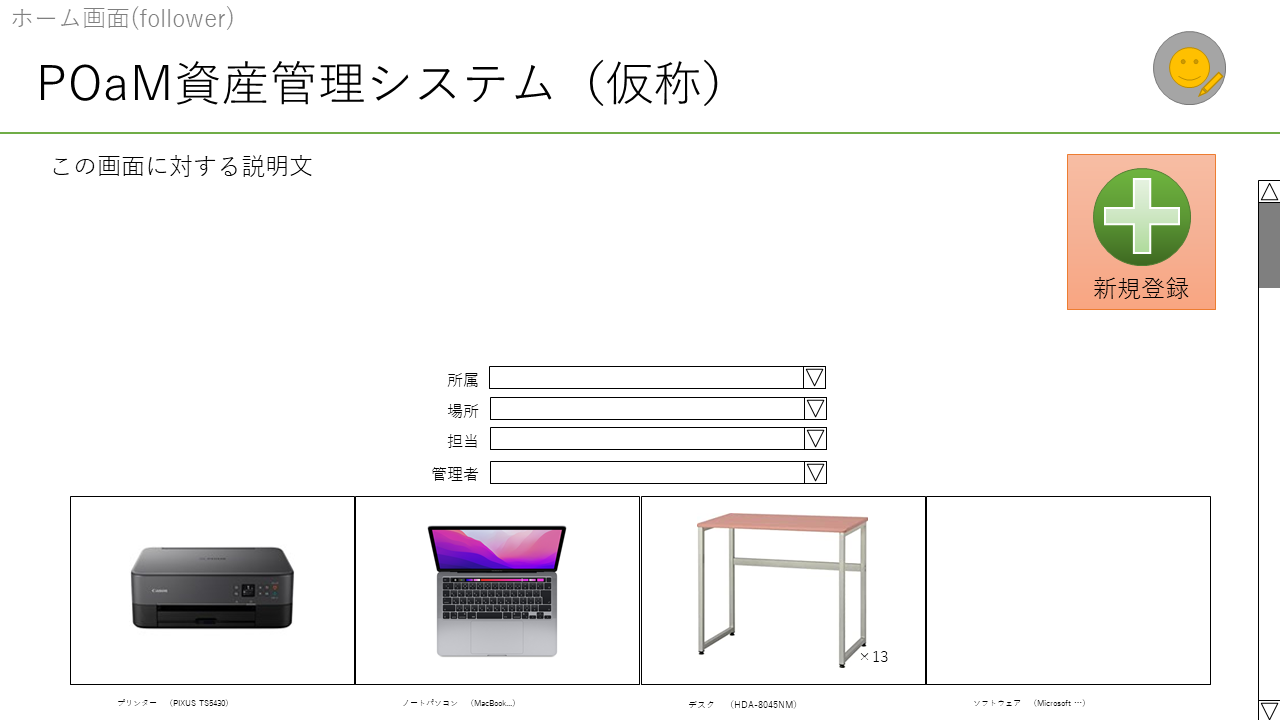
\includegraphics[keepaspectratio, width=0.8\linewidth]{source/home_follower.PNG}
  }
  \caption{\label{fig:ホーム画面(一般ユーザ)のイメージ図}ホーム画面(一般ユーザ)のイメージ図}
\end{figure}
\begin{figure}[h]
  \centering
  \fbox{
    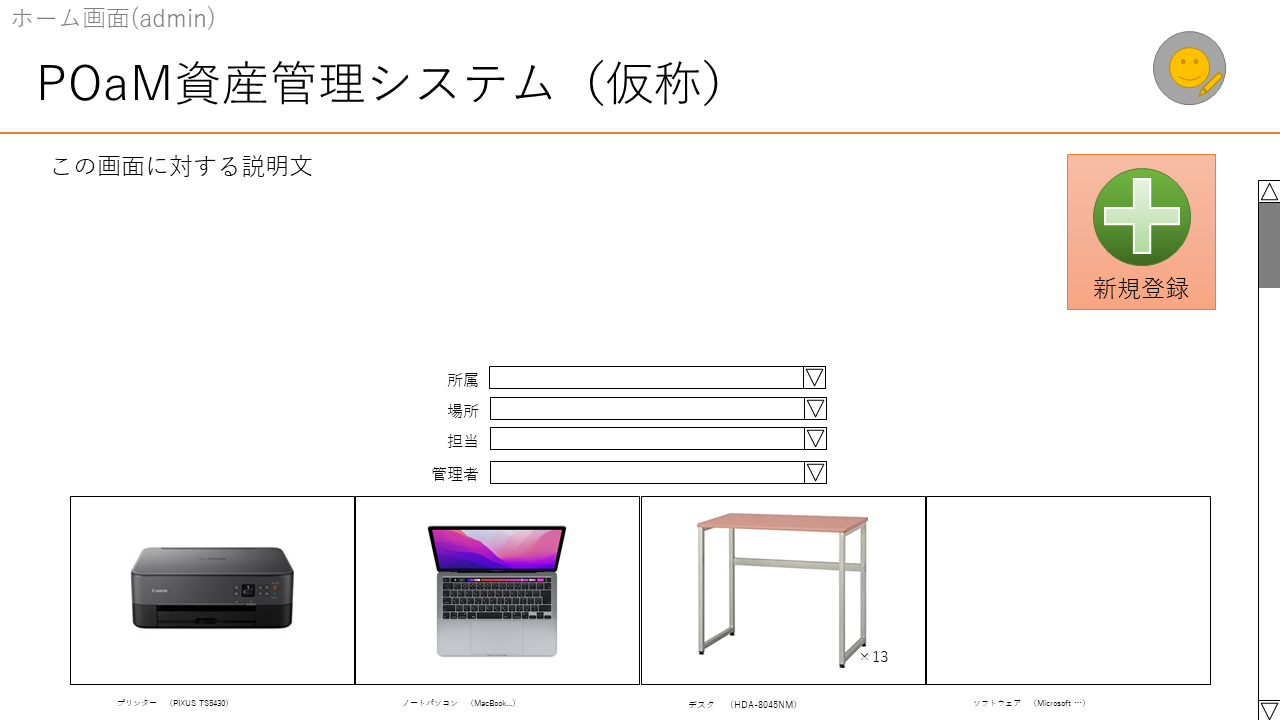
\includegraphics[keepaspectratio, width=0.8\linewidth]{source/home_admin.PNG}
  }
  \caption{\label{fig:ホーム画面(管理者ユーザ)のイメージ図}ホーム画面(管理者ユーザ)のイメージ図}
\end{figure}

%%%%%
\clearpage
\subsubsection{新規登録画面}
\label{sec:新規登録画面}
図\ref{fig:新規登録画面(一般ユーザ)のイメージ図}が一般ユーザ, 図\ref{fig:新規登録画面(管理者ユーザ)のイメージ図}が管理者ユーザに表示される新規登録画面のイメージ図である. \par
ホーム画面(図\ref{fig:ホーム画面(一般ユーザ)のイメージ図}, \ref{fig:ホーム画面(管理者ユーザ)のイメージ図})の「資産登録機能へジャンプするボタン」からジャンプしてきた画面である. \par
各データ項目の入力フォームと, 情報を確定しデータベースへ反映するための完了ボタンがある. 管理者ユーザは一般ユーザよりも入力できる項目が多い. ただし, 所属など一部の項目は入力される内容が限られているため, (例:所属の場合AD, EE, ME, CS, AC)選択式による入力方式を採っている. また, ホーム画面に戻るためのボタンを備えている.
\begin{figure}[h]
  \centering
  \fbox{
    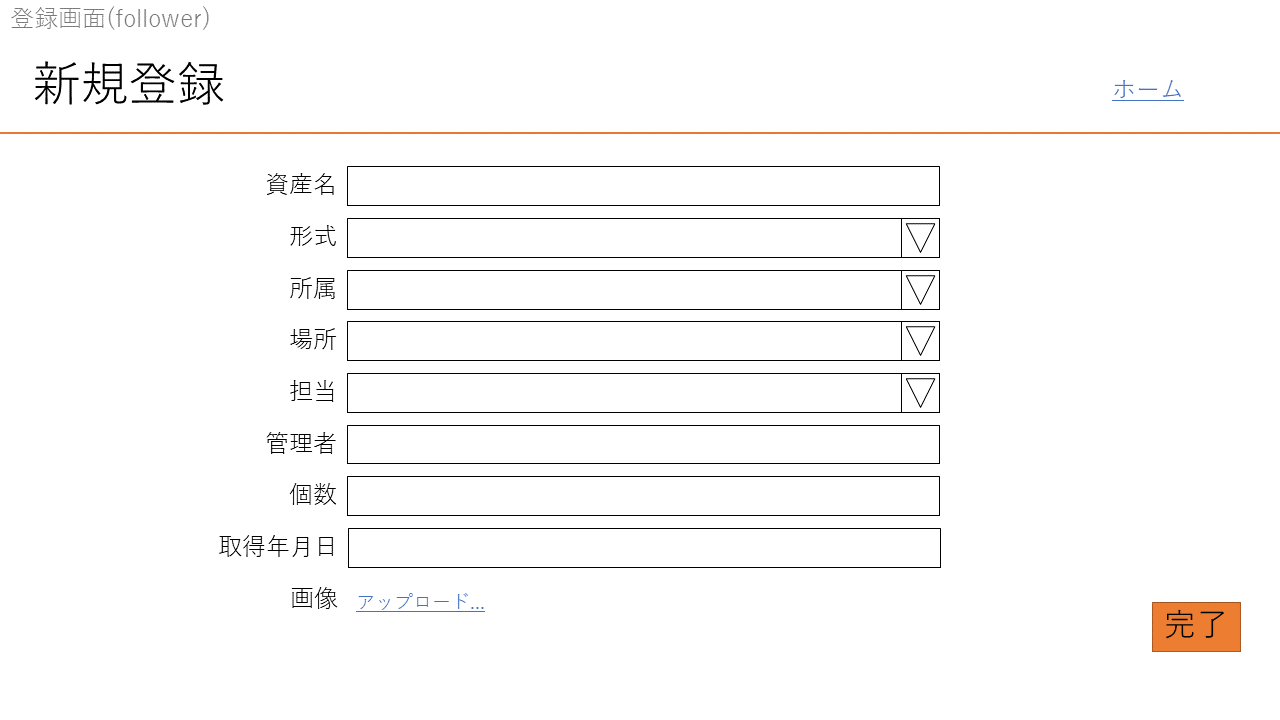
\includegraphics[keepaspectratio, width=0.8\linewidth]{source/submit_follower.PNG}
  }
  \caption{\label{fig:新規登録画面(一般ユーザ)のイメージ図}新規登録画面(一般ユーザ)のイメージ図}
\end{figure}
\begin{figure}[h]
  \centering
  \fbox{
    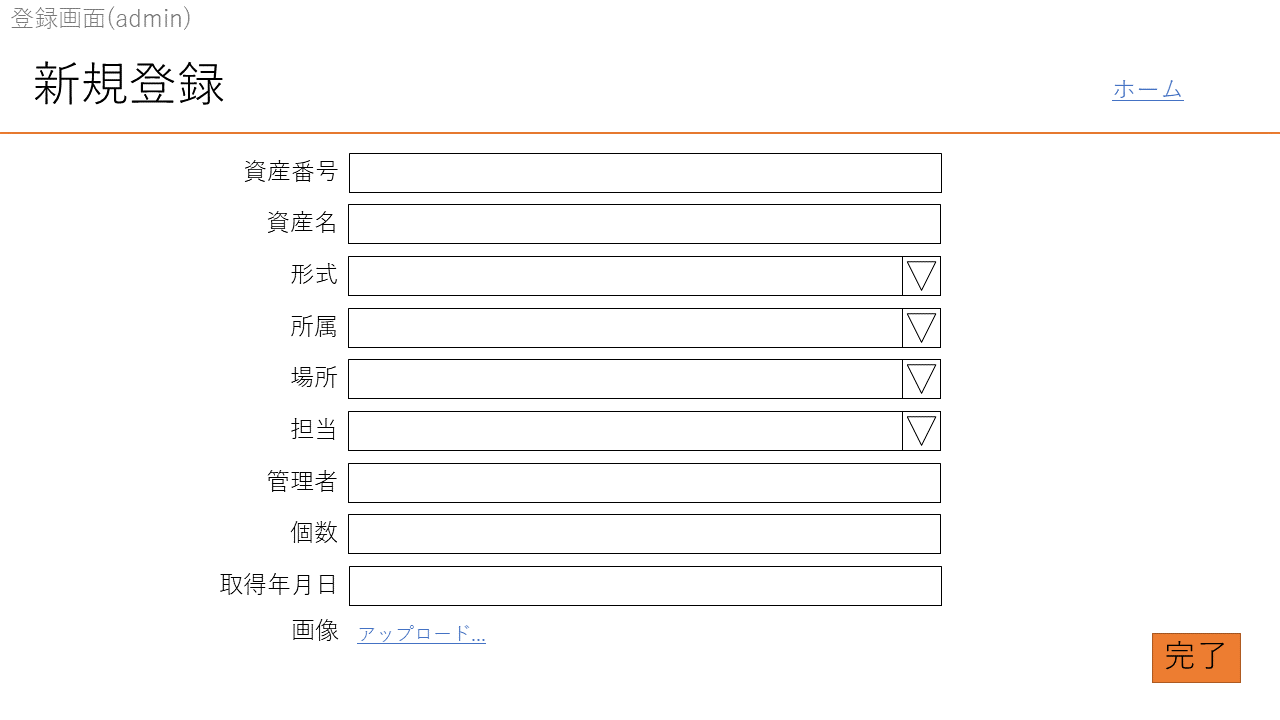
\includegraphics[keepaspectratio, width=0.8\linewidth]{source/submit_admin.PNG}
  }
  \caption{\label{fig:新規登録画面(管理者ユーザ)のイメージ図}新規登録画面(管理者ユーザ)のイメージ図}
\end{figure}

%%%%%
\clearpage
\subsubsection{ユーザ情報編集画面・ユーザ管理画面}
\label{sec:ユーザ情報編集画面・ユーザ管理画面}
図\ref{fig:ユーザ情報編集画面のイメージ図}が一般ユーザ, 図\ref{fig:ユーザ管理画面のイメージ図}が管理者ユーザに表示されるユーザ情報編集画面・ユーザ管理画面のイメージ図である. \par
ホーム画面(図\ref{fig:ホーム画面(一般ユーザ)のイメージ図}, \ref{fig:ホーム画面(管理者ユーザ)のイメージ図})の「ユーザ情報変種機能/ユーザ管理機能へジャンプするボタン」からジャンプしてきた画面である. \par
ユーザ情報編集画面(一般ユーザ)の場合, ログインしているアカウントのID, パスワード, 名前, 所属, アイコンの確認ができる. このうち, パスワードとアイコンが一般ユーザにより任意に変更可能である. また, ホーム画面に戻るためのボタンを備えている. \par
ユーザ管理画面(管理者ユーザ)の場合, システムに存在するアカウントの一覧と, ユーザ新規作成ボタンがある. ユーザの一覧は学科ごとに絞り込みが可能となっている. ユーザ新規作成ボタンおよび各アカウントのエリアは別のページにジャンプする. こちらもホーム画面に戻るためのボタンを備えている. \par
イメージ図は次ページに示す.
\clearpage
\begin{figure}[h]
  \centering
  \fbox{
    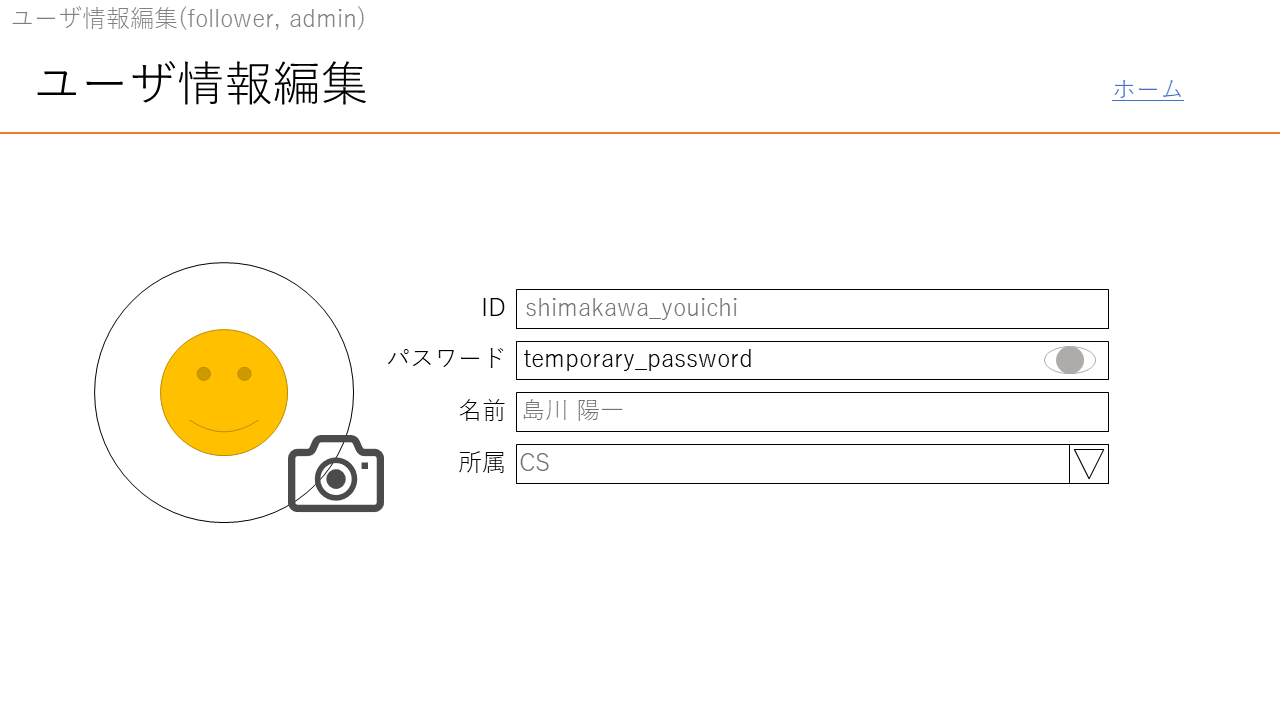
\includegraphics[keepaspectratio, width=0.8\linewidth]{source/user_info_edit_follower.png}
  }
  \caption{\label{fig:ユーザ情報編集画面のイメージ図}ユーザ情報編集画面のイメージ図}
\end{figure}
\begin{figure}[h]
  \centering
  \fbox{
    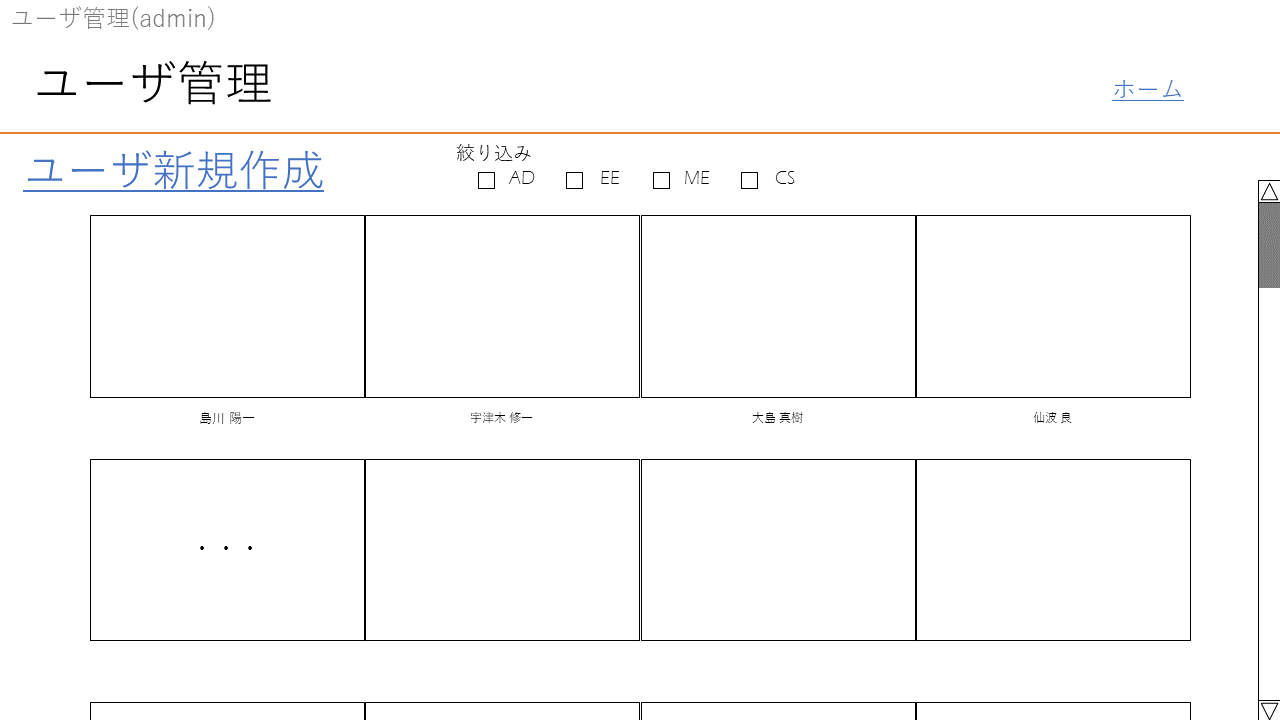
\includegraphics[keepaspectratio, width=0.8\linewidth]{source/user_administration.PNG}
  }
  \caption{\label{fig:ユーザ管理画面のイメージ図}ユーザ管理画面のイメージ図}
\end{figure}

%%%%%
\clearpage
\subsubsection{個別ユーザ管理画面・ユーザ新規作成画面}
\label{sec:個別ユーザ管理画面・ユーザ新規作成画面}
図\ref{fig:個別ユーザ管理画面のイメージ図}が管理者が個別の一般ユーザの情報を編集するための画面, 図\ref{fig:ユーザ新規作成画面のイメージ図}が新規にアカウントを追加するための画面のイメージ図である. \par
個別ユーザ管理画面では、ユーザ管理画面(図\ref{fig:ユーザ管理画面のイメージ図})で選択したアカウントのID, パスワード, 名前, 所属, アイコンの確認ができ(セキュリティの観点からパスワードは閲覧不可)、修正ができる。所属に変更があった場合などに利用する想定である。\par
ユーザ新規作成画面では、ID,名前,所属,アイコンの入力フォームがあり、完了ボタンを押すことで新規のユーザが追加される。ここでユーザが新規作成されることで、そのアカウントにログインすることができるようになる。パスワードは簡単な文字列が初期設定される({\tt password}など想定)。\par
イメージ図は次ページに示す.
\clearpage
\begin{figure}[h]
  \centering
  \fbox{
    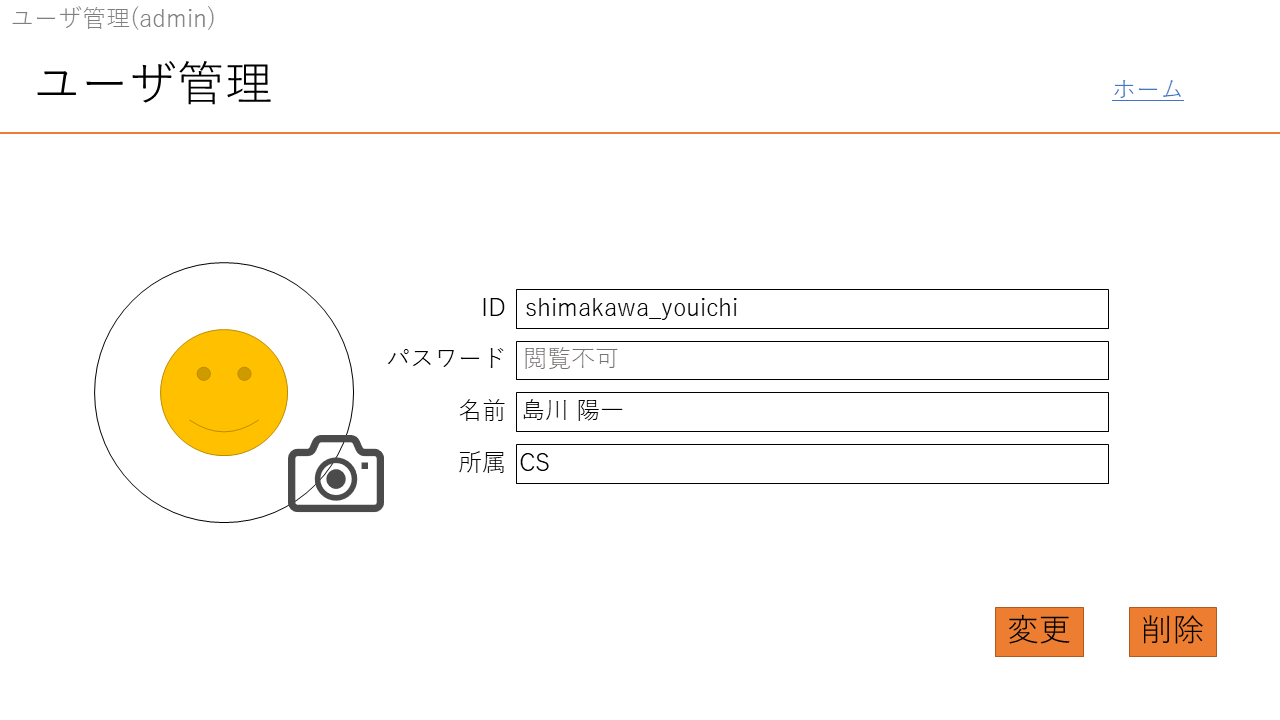
\includegraphics[keepaspectratio, width=0.8\linewidth]{source/user_info_edit_admin.PNG}
  }
  \caption{\label{fig:個別ユーザ管理画面のイメージ図}個別ユーザ管理画面のイメージ図}
\end{figure}
\begin{figure}[h]
  \centering
  \fbox{
    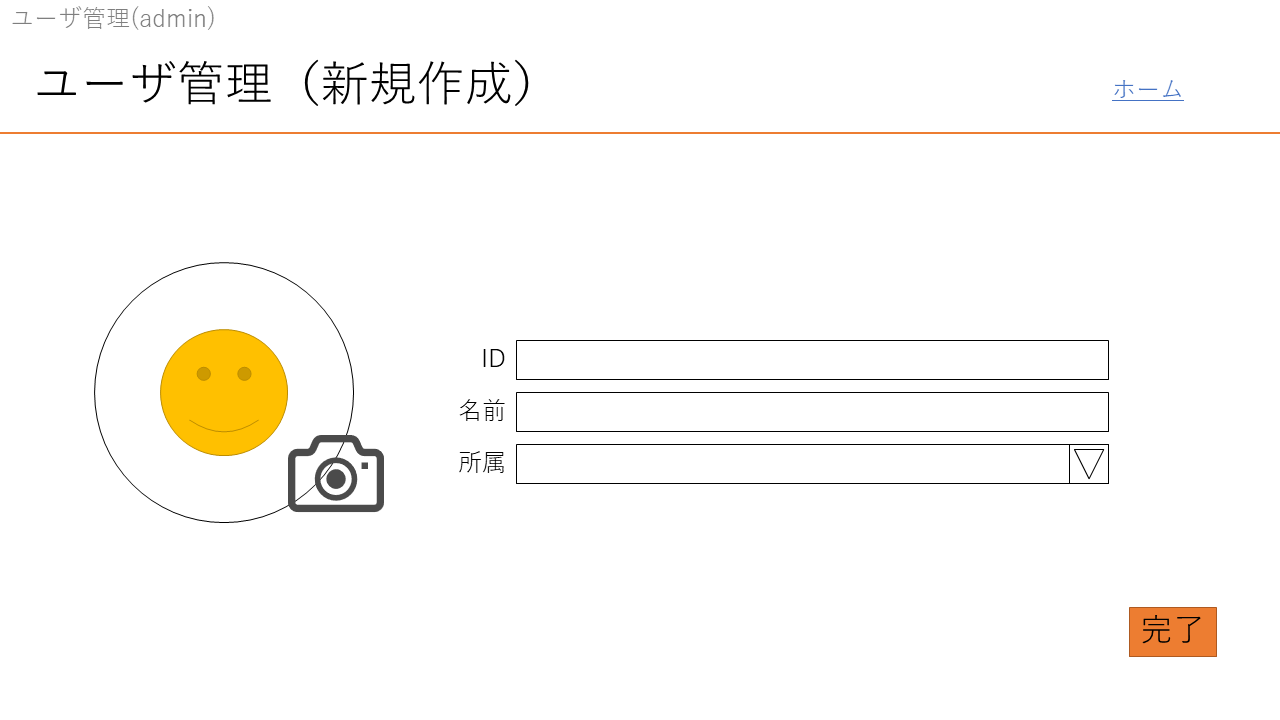
\includegraphics[keepaspectratio, width=0.8\linewidth]{source/user_add.PNG}
  }
  \caption{\label{fig:ユーザ新規作成画面のイメージ図}ユーザ新規作成画面のイメージ図}
\end{figure}

%%%%%
\clearpage
\subsubsection{情報変更画面}
\label{sec:情報変更画面}
図\ref{fig:情報変更画面(一般ユーザ)のイメージ図}が一般ユーザ, 図\ref{fig:情報変更画面(管理者ユーザ)のイメージ図}が管理者ユーザに表示される情報変更画面のイメージ図である. \par
ホーム画面(図\ref{fig:ホーム画面(一般ユーザ)のイメージ図},\ref{fig:ホーム画面(管理者ユーザ)のイメージ図})で選択した資産からジャンプしてきた画面である。\par
一般ユーザの場合、確認は全項目について可能だが、変更できる項目は場所、担当、個数のみに制限されている。\par
管理者ユーザの場合、全項目の確認と変更が可能である。その上、この画面から該当資産データの削除も可能である。
\begin{figure}[h]
  \centering
  \fbox{
    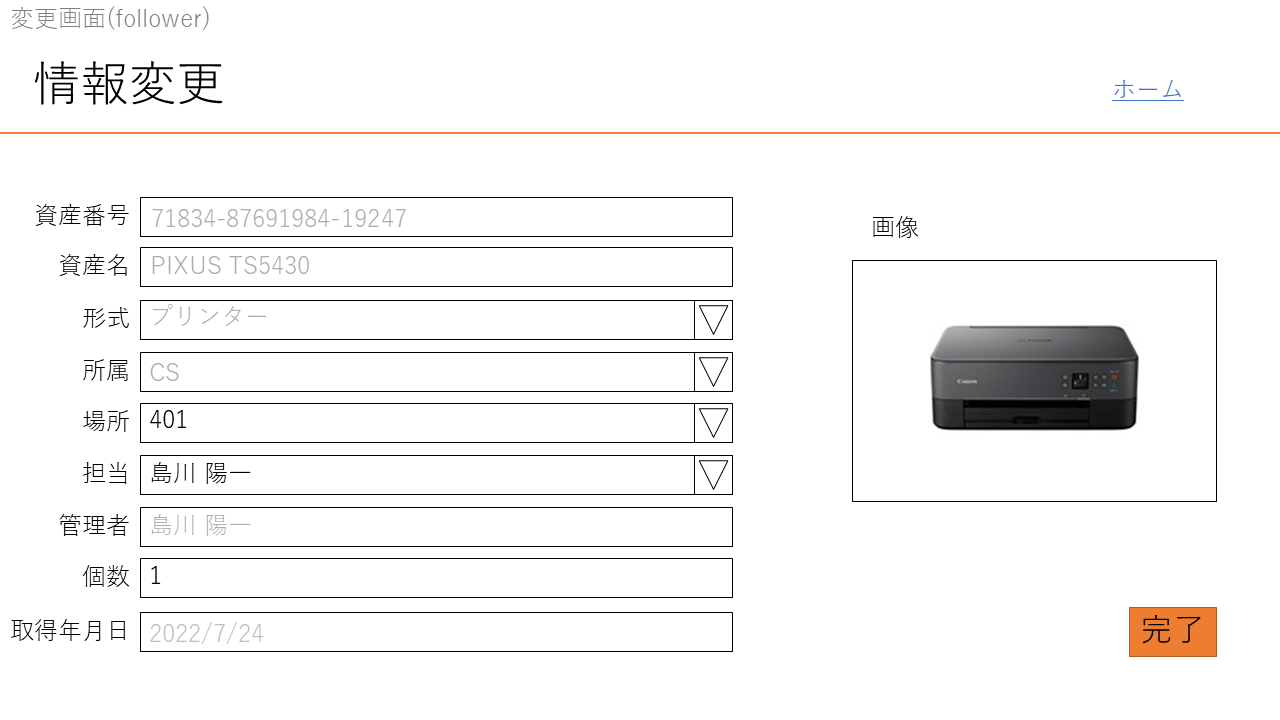
\includegraphics[keepaspectratio, width=0.8\linewidth]{source/change_follower.PNG}
  }
  \caption{\label{fig:情報変更画面(一般ユーザ)のイメージ図}情報変更画面(一般ユーザ)のイメージ図}
\end{figure}
\begin{figure}[h]
  \centering
  \fbox{
    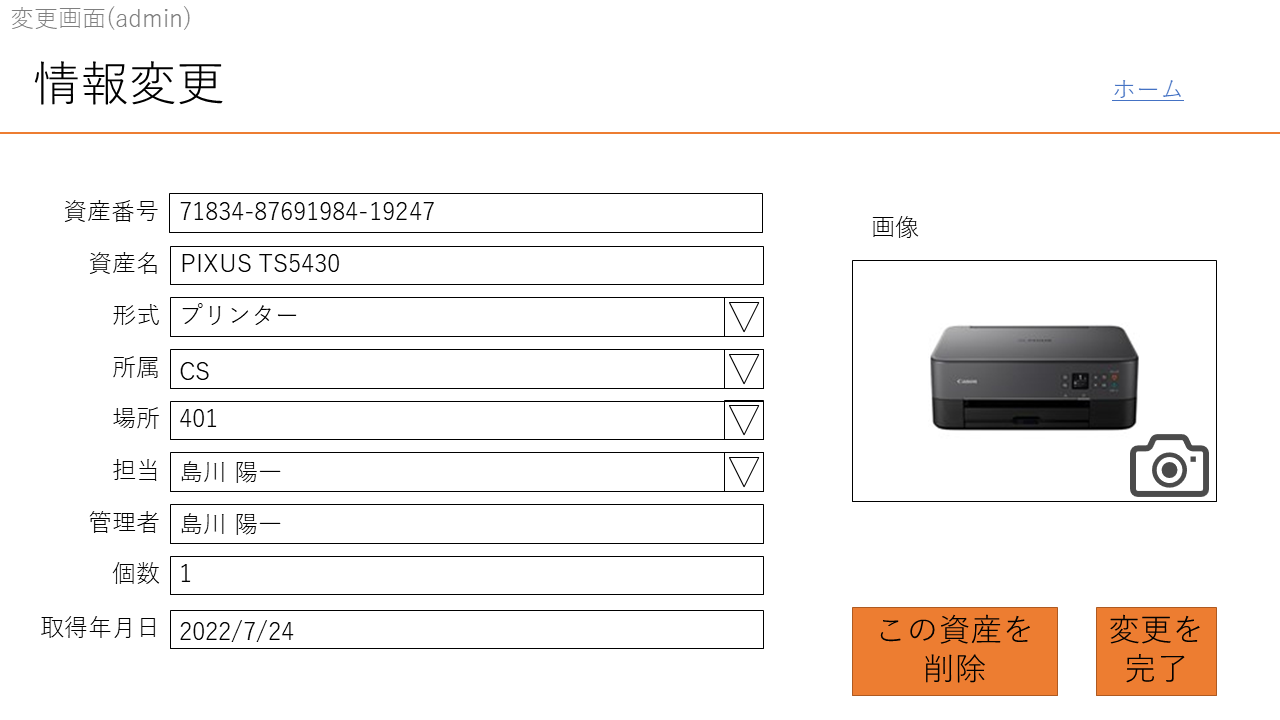
\includegraphics[keepaspectratio, width=0.8\linewidth]{source/change_admin.PNG}
  }
  \caption{\label{fig:情報変更画面(管理者ユーザ)のイメージ図}情報変更画面(管理者ユーザ)のイメージ図}
\end{figure}


%%%%%%%%%%
%\newpage
%\section{用語集}
%\label{sec:用語集}
%\begin{enumerate}
%\item[メールアドレス] @以左のユーザ名(メールアカウント)と, @以右のドメインによって構成される.  例 {\tt test@example.com}
%\end{enumerate}


%%%%%%%%%%
\clearpage
{\Large\bfseries \ 改変履歴}
\begin{table}[htbp]
  %\caption{}
  %\label{tb:}
  \centering
  \begin{tabularx}{\textwidth}{wc{0.2\linewidth}|wl{0.6\linewidth}|wl{0.2\linewidth}}
    日付       & 項目                                           & 担当者     \\
    \hline \hline
    2022/05/27 & 初版作成                                       & 田桑       \\
    \hline
    2022/06/09 & 全体の表現の変更・追加                         & 高橋・田中 \\
    \hline
    2022/07/05 & \ref{sec:各機能の詳細・システムの詳細}節の編集 & 高橋・田中 \\
    \hline
    2022/07/21 & \ref{sec:各機能の詳細・システムの詳細}節の編集 & 高橋・田中 \\
    \hline
    2022/11/30 & \ref{sec:各機能の詳細・システムの詳細}節の編集 & 高橋・田中 \\
    \hline
    2022/12/01 & \ref{sec:各機能の詳細・システムの詳細}節の編集 & 高橋・田中 \\
    % \hline
  \end{tabularx}
\end{table}


\end{document}
%%%%%%%%%%%%%%%%%%%
%%%%%%%%%%%%%%%%%%%

%
